\chapter{ヒッグススケール、走る結合定数、そして階層性問題}

\lectureoverview{最終講義は、標準模型を超えて統一、超対称性、ゲージ階層性問題へと目を向けることから始まる。ヒッグス場がなぜこれらの問いの中心に位置するのかを見るために、まずディラックラグランジアンを再構成し、フェルミオンの質量が左巻きと右巻きのカイラリティを混合することを示す。カイラルな弱い相互作用はその質量を裸の項として禁じる。ゲージ不変な湯川結合は、ヒッグス場が真空期待値を獲得した後に初めてそれを供給する。次にその真空期待値をヒッグスポテンシャルから導出し、なぜ既知のすべての素粒子質量がこの一つの小さなスケールに結びついているのかを問い、超伝導を物理的類推として用いる。対称性の破れの後、講義は伝導体と誘電体の遮蔽から繰り込みを展開し、その議論をQEDとQCDへと運び、ゲージ結合定数を統一へと追い、短距離重力からプランクスケールを導出する。そして電弱スケールが、唯一説明されない小さな数として再び戻ってくる。}

\section{標準模型の先に待つ問い}

標準模型はここで閉じた目録として提示されるものではない。今夜の冒頭で、次の講義がどこへ向かうのかを述べておきたい。この理論には論理的パラドックスではなく困難がある。ゲージ階層性、超対称性が果たしうる役割、そして統一の問題である。三つのゲージ因子
\begin{equation}
  SU(3)_c\times SU(2)_L\times U(1)_Y
  \label{eq:l10-standard-model-group}
\end{equation}
は強い相互作用、弱い相互作用、ハイパーチャージ相互作用を別々に記述する。それらは一つのより大きな群の部分群でありうるだろうか。しばしば研究される可能性は
\(SU(5)\)
であり、その中でクォークとレプトンは共通の多重項を占める。自然がその特定の構成を用いているかどうかは別の問題である。重要な手がかりは、見かけ上別々の構造が、驚くほどきれいに一つのより大きな数学的構造に収まるということである。

大型ハドロン衝突型加速器は、これらの問いを決着させる物理学を明らかにするために、部分的に建設された。2010年において、その最も直接的な獲物はヒッグス粒子であった。ヒッグス粒子の発見は、決して表に一つの粒子を加えることだけを意味しえなかった。ヒッグス粒子は相互に連関する性質の集合によって同定される。その真空期待値は弱ゲージベクトルボソンとフェルミオンに質量を与え、その揺らぎはそれら同じ粒子と確定した強さで結合する。誤った結合を持つ共鳴は標準模型のヒッグス粒子ではない。\editorialnote{この講義は2012年の発見に先立つものである。観測されたおよそ\(125\,\mathrm{GeV}\)のスカラーは、現在の精度の範囲内で、標準模型のヒッグス粒子に期待されるスピン、パリティ、結合のパターンを持つ。2026年時点で、低エネルギーの超対称粒子は観測されていない。これらの後知恵の事実は、その場で展開された議論を変えることなく、歴史的状況を更新するものである。}

その議論への道は、ヒッグスポテンシャルではなくディラック方程式から始まる。フェルミオンの質量が正確に何をするのかを、それがどこから来るのかを問う前に理解する必要がある。

\section{ディラック方程式からそのラグランジアンへ}

\subsection{古いディラック記法}

ディラック方程式が最初に導入されたときに用いられたハミルトニアン記法では、その構造は
\begin{equation}
  i\partial_t\psi
  =
  \left(-i\alpha^i\partial_i+\beta m\right)\psi .
  \label{eq:l10-dirac-hamiltonian}
\end{equation}
である。符号と\(i\)の因子は規約に依存し、生の黒板ではその一部が一時的に省略されている。不変な内容は、微分を含む項と、微分を含まない質量項との分離である。

\begin{figure}[htbp]
\centering
\includegraphics[width=0.82\textwidth]{lecture_10_figure_02.png}
\caption{古い\(\alpha,\beta\)記法におけるディラック方程式とラグランジアン。黒板は固定された符号規約としてではなく、構造的に用いられている。}
\lectureframe{00:05:52}
\label{fig:l10-dirac-alpha-beta}
\end{figure}

変分がディラック方程式を与える作用を得るには、方程式に\(\psi^\dagger\)を掛ける。すべての項を一方の辺に移せば等号の必要がなくなり、今夜の小さな数学的冗談を引き起こす。すなわち、方程式がゼロに等しい式として書かれてしまえば、等号はその役目を終えている。対応する一階のラグランジアンは模式的に
\begin{equation}
  \mathcal L
  =
  \psi^\dagger
  \left(i\partial_t+i\alpha^i\partial_i-\beta m\right)\psi ,
  \label{eq:l10-dirac-old-lagrangian}
\end{equation}
と書くことができ、整合的な計量規約が相対符号を固定するものと理解される。

微分項は励起を一つの時空点から近傍の点へと移し、その過程でそのスピノル成分を回転させる。格子の描像では、これらはホッピング項である。対照的に、質量項はフェルミオンを同じ点で吸収し再放出する。微分を持たない。この局所的操作は、まもなく二種類の巻き性の間の繰り返される変換として自らを明らかにするだろう。

\begin{classroomqa}
\audiencequestion{\(\gamma^0\)は
\(\psi^\dagger\)の後に置くべきか。\lecturetimestamp{00:05:59}}
\lecturerresponse{いま書いた非共変形式ではそうではない。しかし、この問いは共変記法を直接指し示している。ディラック共役を\(\bar\psi=\psi^\dagger\gamma^0\)で定義すれば、\(\gamma^0\)は確かに左側に立つ対象に組み込まれている。}
\end{classroomqa}

\subsection{共変形式}

\begin{equation}
  \bar\psi\equiv\psi^\dagger\beta
  =\psi^\dagger\gamma^0,
  \qquad
  \gamma^0\equiv\beta,
  \qquad
  \gamma^i\equiv\beta\alpha^i .
  \label{eq:l10-dirac-adjoint}
\end{equation}
を設定する。\(\beta^2=1\)であるから、\(\beta\)を掛けることで二つの記法の間を自由に変換できる。時間微分は
\(\bar\psi\gamma^0\partial_0\psi\)となり、空間微分は
\(\bar\psi\gamma^i\partial_i\psi\)となり、結果は
\begin{equation}
  \boxed{\mathcal L_D
  =\bar\psi\left(i\gamma^\mu\partial_\mu-m\right)\psi .}
  \label{eq:l10-covariant-dirac}
\end{equation}となる。

\begin{figure}[htbp]
\centering
\includegraphics[width=0.82\textwidth]{lecture_10_figure_03.png}
\caption{共変形への書き換え：\(\bar\psi=\psi^\dagger\gamma^0\)、
\(\gamma^i=\beta\alpha^i\)、そしてコンパクトなディラックラグランジアン。}
\lectureframe{00:10:17}
\label{fig:l10-dirac-covariant}
\end{figure}

この記法は各双線形のローレンツ的性質を露わにする。
\(\bar\psi\psi\)はスカラーであるのに対し、
\(\bar\psi\gamma^\mu\psi\)は四元ベクトルである。コンパクトな表式は\(\alpha,\beta\)の形式よりも単に美しいだけでなく、各部分がどのように変換するかを教えてくれる。

\begin{classroomqa}
\audiencequestion{コンパクトな表式の最も左にあるスピノルは\(\bar\psi\)のつもりだったのか。\lecturetimestamp{00:09:39}}
\lecturerresponse{はい。欠けていたバーは板書で復元される。これは重要である：
\(\bar\psi\)は\(\psi^\dagger\)ではなく、
\(\psi^\dagger\gamma^0\)である。}
\end{classroomqa}

\section{カイラリティとディラック質量が実際に行うこと}

\(\gamma^0,\gamma^1,\gamma^2,\gamma^3\)に加えて、
\begin{equation}
  \gamma^5
  =i\gamma^0\gamma^1\gamma^2\gamma^3,
  \qquad
  (\gamma^5)^2=1 .
  \label{eq:l10-gamma-five}
\end{equation}
を定義する。ここに示した\(i\)の因子は、主にマイナスのミンコフスキー計量に対する標準的な規約である。固有値は\(+1\)と\(-1\)であり、対応する射影演算子は
\begin{equation}
\begin{aligned}
  P_L&=\frac{1-\gamma^5}{2},
  &
  P_R&=\frac{1+\gamma^5}{2},
  \\
  \psi_L&=P_L\psi,
  &
  \psi_R&=P_R\psi .
\end{aligned}
  \label{eq:l10-chiral-projectors}
\end{equation}である。

\begin{classroomqa}
\audiencequestion{\(\gamma^4\)が存在しないのに、なぜ余分な行列は\(\gamma^5\)と呼ばれるのか。そしてその固有値はヘリシティを表すのか。\lecturetimestamp{00:10:42}}
\lecturerresponse{名前は歴史的なものである：それは四つの時空ガンマ行列の積から作られる追加の行列である。その固有値はカイラリティを標識し、一般にはヘリシティではない。質量のない粒子に対しては二つの概念を適切に同一視できるため、言葉が混同されやすいが、カイラリティは弱ゲージ理論が必要とするローレンツ表現のラベルである。}
\end{classroomqa}

運動項はカイラリティを保存する。これを見る有用な方法の一つは
\(\{\gamma^\mu,\gamma^5\}=0\)であるから、
\begin{equation}
  \bar\psi i\gamma^\mu\partial_\mu\psi
  =
  \bar\psi_L i\gamma^\mu\partial_\mu\psi_L
  +
  \bar\psi_R i\gamma^\mu\partial_\mu\psi_R .
  \label{eq:l10-chiral-kinetic}
\end{equation}
に分離することである。スカラー双線形は異なる振る舞いをする：
\begin{equation}
  \bar\psi\psi
  =
  \bar\psi_L\psi_R+\bar\psi_R\psi_L .
  \label{eq:l10-chiral-mass}
\end{equation}

\begin{figure}[htbp]
\centering
\includegraphics[width=0.80\textwidth]{lecture_10_figure_04.png}
\caption{板書はスカラー双線形を左から右への部分と右から左への部分に分解する。}
\lectureframe{00:15:38}
\label{fig:l10-chiral-decomposition}
\end{figure}

したがってディラック質量は局所的なカイラリティ反転操作である：
\begin{equation}
  \psi_L\longleftrightarrow\psi_R .
\end{equation}
質量のないフェルミオンは確定したカイラリティで伝播してよい。質量のあるフェルミオンは一つのカイラルセクターにとどまることができない。質量項が絶えず二つを混合するからである。この変換が慣性と何か関係があるとは意外に思われるかもしれないが、これはまさにフェルミオンの静止質量の相対論的場の理論的表現である。

\section{なぜ弱対称性は裸のフェルミオン質量を禁じるのか}

荷電弱カレントは純粋に左巻きカイラルである。講義はまず\(Z\)と述べ、次にその記述を\(W^\pm\)へと訂正する：\(Z\)結合はカイラルであり等しくないが、すべての右巻きカイラルフェルミオンに対して単に存在しないわけではない。明確な記述は
\begin{equation}
  \mathcal L_{\mathrm{cc}}
  =
  -\frac{g}{\sqrt2}
  \left(\bar u_L\gamma^\mu d_L
  +\bar\nu_L\gamma^\mu e_L\right)W^+_\mu
  +\mathrm{h.c.}
  \label{eq:l10-charged-current}
\end{equation}
である。左巻きフェルミオンは\(SU(2)_L\)二重項として変換し、右巻き荷電フェルミオンは一重項として変換する。

次にこれらの変換則を
\eqref{eq:l10-chiral-mass}と比較する。
\(\bar e_L e_R\)のような項は、一組の電気弱量子数を持つ対象を吸収し、別のものを持つ対象を放出する。それ自体ではゲージ不変ではない。したがって、おなじみのディラック質量は電気弱ラグランジアンにおける裸の項としては許されない。

これは説明の正しい順序である。フェルミオン質量はまず挿入され、その後で見かけ上ヒッグスと結び付けられるのではない。ゲージ対称性がまず明白な質量項を排除する。次にヒッグス場が、欠けている量子数を担うことを強いられる。

\subsection{電荷を担うものとしてのヒッグス}

ヒッグスがハイパーチャージ
\(+\tfrac12\)を持つ\(SU(2)_L\)二重項として変換するとしよう：
\begin{equation}
  H=
  \begin{pmatrix}
    H^+\\ H^0
  \end{pmatrix},
  \qquad
  \widetilde H=i\sigma^2H^* .
  \label{eq:l10-higgs-doublet}
\end{equation}
講義は群指数を模式的に保ち、場を\(\phi\)と呼ぶ。その記法では、湯川項は
\begin{equation}
  \mathcal L_Y
  =
  -G_Y\left(
    \bar\psi_L\phi\psi_R+
    \bar\psi_R\phi^\dagger\psi_L
  \right).
  \label{eq:l10-yukawa-schematic}
\end{equation}
の形をとる。ヒッグス場は、裸のカイラリティ反転では保存できない弱電荷を持ち去る。

一世代の標準模型の完全な表式は同じ帳尻合わせを明示する：
\begin{equation}
  \mathcal L_Y
  =
  -y_d\bar Q_LHd_R
  -y_u\bar Q_L\widetilde H u_R
  -y_e\bar L_LHe_R
  +\mathrm{h.c.}
  \label{eq:l10-yukawa-full}
\end{equation}
各項はゲージ不変であり、各フェルミオン種はそれぞれ自身の無次元湯川結合を持つ。

\begin{figure}[htbp]
\centering
\includegraphics[width=0.80\textwidth]{lecture_10_figure_05.png}
\caption{ヒッグスに助けられたカイラリティ反転と対称性の破れのポテンシャルが板書に一緒に現れる。}
\lectureframe{00:18:54}
\label{fig:l10-yukawa-potential-board}
\end{figure}

\section{一つの相互作用が質量とヒッグス結合の両方になる}

自然は、中性ヒッグス成分が消えない真空を選ぶ。講義で用いられた模式的な実場の記法では、
\begin{equation}
  \phi=F+\mathcal H ,
  \label{eq:l10-f-plus-h}
\end{equation}
ここで\(F\)は揺らがない真空のずれであり、\(\mathcal H\)は伝播するヒッグス揺らぎである。\eqref{eq:l10-yukawa-schematic}に代入すると
\begin{align}
  \mathcal L_Y
  ={}&
  -G_YF
  \left(\bar\psi_L\psi_R+\bar\psi_R\psi_L\right)
  \notag\\
  &-G_Y\mathcal H
  \left(\bar\psi_L\psi_R+\bar\psi_R\psi_L\right).
  \label{eq:l10-yukawa-split}
\end{align}
が得られる。第1行はディラック質量であり、第2行は物理的なヒッグス量子との相互作用である：
\begin{equation}
  m_f=G_YF
  \qquad\hbox{in the lecture's normalization.}
  \label{eq:l10-mass-lecture-normalization}
\end{equation}

従来の標準模型の規格化では、
\begin{equation}
\begin{aligned}
  H(x)&=\frac{1}{\sqrt2}
  \begin{pmatrix}
    0\\ v+h(x)
  \end{pmatrix},
  \\
  m_f&=\frac{y_fv}{\sqrt2},
  \\
  \mathcal L_{hff}&=-\frac{m_f}{v}h\bar f f,
\end{aligned}
  \label{eq:l10-standard-higgs-normalization}
\end{equation}
であり、\(v\simeq246\,\mathrm{GeV}\)である。講義の粗い\(F\sim200\,\mathrm{GeV}\)は、規格化の詳細を省いたこの同じ電弱スケールである。

測定された\(W\)および\(Z\)の質量がスケール\(F\)を決める。次に測定されたフェルミオン質量が湯川結合を決める。電子の結合はごく小さく、トップクォークの結合は1の程度である。もし機構がこれだけを行うなら、フェルミオンごとに1つの未知数を入れて、同じ情報をそのまま読み出しただけになるだろう。

しかし\eqref{eq:l10-yukawa-split}の第2行は新しい実験的内容である。それは、フェルミオンがヒッグスを放出または吸収できること、そして交差チャネルで読めば、ヒッグスがフェルミオン・反フェルミオン対に崩壊できることを述べている。模式的には、
\begin{equation}
\begin{aligned}
  \mathcal M(h\to f\bar f)&\propto y_f,
  \\
  \Gamma(h\to f\bar f)
  &=
  N_c\frac{y_f^2m_h}{16\pi}
  \\
  &\quad\times
  \left(1-\frac{4m_f^2}{m_h^2}\right)^{3/2},
\end{aligned}
  \label{eq:l10-higgs-fermion-width}
\end{equation}
がツリーレベルで成り立つ。ここでクォークでは\(N_c=3\)、レプトンでは\(1\)である。崩壊が運動学的に許されるならば、より大きなフェルミオン質量はより大きな湯川結合を意味する。これは、すべての重いチャネルが支配的であることを意味しない。カラーの因子、位相空間、ループ誘起チャネル、ベクトルボソンへの崩壊も重要である。そうではなく、フェルミオン結合自体が質量に比例することを意味する。

\begin{classroomqa}
\audiencequestion{ヒッグス粒子の崩壊時間を、技術的な細部をすべて計算することなく、実際にどのように予測するのだろうか。\lecturetimestamp{00:25:32}}
\lecturerresponse{相互作用はハミルトニアン行列要素を与える。対応するファインマン図を描き、その遷移振幅を計算し、振幅を二乗し、許されるすべての終状態について和または積分を行う。その結果が崩壊率である。寿命は全幅の逆数、\(\tau=\hbar/\Gamma_{\mathrm{tot}}\)である。これは、量子場の理論の初期の発展以来、素粒子計算で用いられてきたのと同じ量子力学の論理である。}
\end{classroomqa}

講義の時点では、このヒッグス現象論はまだ直接観測ではなく予測であった。\(W\)および\(Z\)の自己相互作用はすでにゲージ構造の厳しい検証を与えていたが、ヒッグスとその直接的結合は見つかるべきものとして残っていた。歴史的な不確かさは記録に属する。その後の結果も同様である。ヒッグスに似た粒子が見つかり、その結合の測定は今や、ここで展開された同じ質量生成構造の検証となっている。

\section{Fを選ぶポテンシャル}

真空のずれは、湯川結合を書いた後に手で選ばれるのではない。それはヒッグスポテンシャルによって決定される。完全な二重項を通る1つの実断面について、
\begin{equation}
  V(\phi)
  =
  -\frac{\mu^2}{2}\phi^2
  +\frac{\lambda}{4}\phi^4,
  \qquad
  \mu^2>0,\quad\lambda>0.
  \label{eq:l10-real-higgs-potential}
\end{equation}
\(\phi=0\)の近くでは、負の二次項が上下逆さまの放物線をつくる。\(\mu\)を虚数質量と呼ぶのは、原点が不安定であることを言い換えたものであり、真の真空のまわりの物理的ヒッグス励起が虚数質量をもつという意味ではない。

二次項だけでは場は際限なく駆動され、最低エネルギー状態が残らない。正の四次項がやがて支配的になり、ポテンシャルを上向きに変える。奇数次の項はおもちゃの\(\phi\mapsto-\phi\)対称性を損なう。四次項は最初の偶数の安定化相互作用であり、4次元時空では、無次元結合をもつ最高次の多項式スカラー相互作用である。

微分すると：
\begin{align}
  \frac{dV}{d\phi}
  &=-\mu^2\phi+\lambda\phi^3
  \notag\\
  &=\phi\left(-\mu^2+\lambda\phi^2\right).
  \label{eq:l10-potential-derivative}
\end{align}
停留点\(\phi=0\)は不安定な頂上である。2つの極小は、この実場の規約で
\begin{equation}
  \boxed{F^2=\frac{\mu^2}{\lambda}},
  \qquad
  F=\frac{\mu}{\sqrt\lambda}
  \label{eq:l10-vacuum-value}
\end{equation}
を満たす。

\begin{figure}[htbp]
\centering
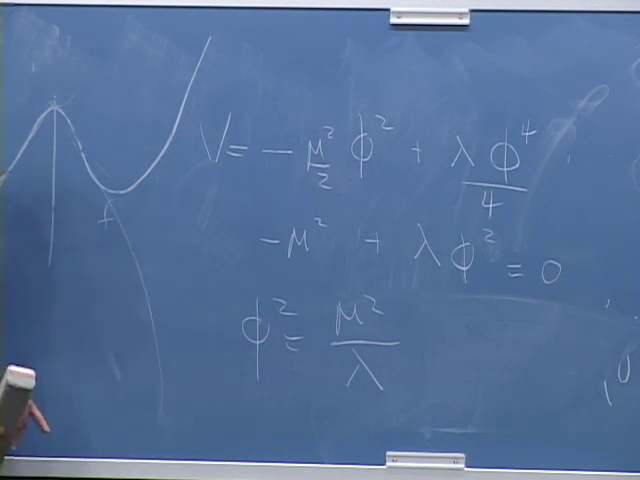
\includegraphics[width=0.84\textwidth]{lecture_10_figure_06.png}
\caption{黒板での最小化の完成：
\(V=-\mu^2\phi^2/2+\lambda\phi^4/4\)、
\(V'=0\)、そして\(\phi^2=\mu^2/\lambda\)。}
\lectureframe{00:34:32}
\label{fig:l10-higgs-minimization}
\end{figure}

因子\(1/2\)と\(1/4\)は、微分するとちょうど消えるように挿入された。原点の近くでは\(\phi^4\)は\(\phi^2\)より小さく、大きな場ではより速く成長して系を安定化する。この単純な競合が二重井戸を生む。

次元もまた、記録中の一時的な口頭の言い間違いを解決する。\(\lambda\)は4次元時空で無次元であり、一方\(\mu\)と\(F\)は質量の次元をもつ。\(\phi=F+\mathcal H\)を展開すると、ポテンシャルの曲率は
\begin{equation}
  m_{\mathcal H}^2
  =
  \left.\frac{d^2V}{d\phi^2}\right|_{\phi=F}
  =
  -\mu^2+3\lambda F^2
  =
  2\mu^2
  =
  2\lambda F^2.
  \label{eq:l10-higgs-curvature}
\end{equation}
を与える。完全な標準模型の記法\(V(H)=-\mu^2H^\dagger H+\lambda(H^\dagger H)^2\)でも同様に
\(m_h^2=2\lambda v^2\)
が成り立つ。測定されたヒッグス質量と\(v\)は、電弱スケールで\(0.13\)付近の\(\lambda\)を意味する。講義の2010の見積もりは意図的に粗く、構造的な主張は\(\lambda\)が不合理に小さな数ではないということであった。

\section{なぜ我々が見るものすべてがこのスケールに結びついているのか。}

同じ\(F\)が\(W\)と\(Z\)の質量を支配し、異なる湯川結合を掛けることで、すべての荷電フェルミオンの質量をも支配する。この経験的な集中は、代数よりも興味深い問いを提起する。なぜ既知の素粒子はすべて、同じ対称性の破れという現象から質量を借りなければならないのか。

ありうるすべての粒子がそうしなければならないという定理は存在しない。左巻き成分と右巻き成分がゲージ群の下で同じように変換するベクトル的フェルミオンを想像しよう。そのとき\(\bar\psi_L\psi_R+\mathrm{h.c.}\)はヒッグスなしでゲージ不変でありうる。完全なゲージ一重項も同様に、電弱の破れとは無関係な質量を持つことができる。そのような粒子は、\(F\)に結びついた粒子よりも自然にずっと重くなりうる。われわれが発見した粒子が目に見えるほど軽いのは、まさに\(F\)が消えるとき対称性がそれらを質量ゼロにするからかもしれない。

したがって電弱スケールが例外的な数である。 speculativeな描像は、保護されていない一般的な質量ははるかにより大きな基礎スケールの近くにあり、一方でカイラルゲージ対称性によって保護された粒子は\(F\)とともに引きずり下ろされるというものである。

\begin{classroomqa}
\audiencequestion{プランク質量は、\(F\)と比較すべき基礎質量スケールの候補の一つか。\lecturetimestamp{00:38:43}}
\lecturerresponse{はい。もう一つは、ゲージ結合の統一によって示唆されるスケールである。それらの巨大な質量の粒子は直接観測されていないが、どちらも講義の後半の議論から現れるであろう。}
\end{classroomqa}

\begin{classroomqa}
\audiencequestion{他のスケールが\(F\)より約15桁上にあるとはどういう意味か、そしてそれらにはどの粒子が対応するのか。\lecturetimestamp{00:39:54}}
\lecturerresponse{電弱スケールは\(10^2\,\mathrm{GeV}\)の程度であり、一方で統一は\(10^{16}\,\mathrm{GeV}\)付近で示唆され、プランクスケールは\(10^{19}\,\mathrm{GeV}\)付近にある。われわれはそれらの質量の粒子を生成していない。スケールは間接的に推論する。一つは測定されたゲージ結合の外挿から、もう一つは量子力学、相対性理論、ニュートンの定数を組み合わせることからである。}
\end{classroomqa}

\section{実験室における荷電凝縮体}

休憩の前に、聴衆からの質問がヒッグス機構の通常の凝縮系類似物を求める。答えは単なる類推だけではなく、段階を追って展開される。

\begin{classroomqa}
\audiencequestion{極低温ボース凝縮体以外に、ヒッグス的な機構の一般的な固体の例はあるか。\lecturetimestamp{00:40:50}}
\lecturerresponse{はい。中性のボース場はボース凝縮体や超流動体において非零の期待値を獲得しうる。凝縮した対象が荷電であれば、同じ基本的現象がゲージ場を変化させる。超伝導がよく知られた例を与える。荷電クーパー対が凝縮し、電磁場は物質内部で有限の侵入長を獲得する。}
\end{classroomqa}

分子分解能では、ヘリウム原子は場\(\Phi_{\mathrm{He}}\)を持つ一つの有効ボース粒子として扱うことができる。空の空間は場がゼロに対応し、超流動相は\(\langle\Phi_{\mathrm{He}}\rangle\ne0\)を持ち、関連する大域的位相対称性を自発的に破る。ヘリウム原子は中性であるため、これはまだゲージ場の質量機構ではない。

超伝導体では、電子は弱く束縛されたクーパー対を形成する。対の場は模式的には電子の双線形であり、
\begin{equation}
  \Delta(x)\sim\langle\psi_\downarrow(x)\psi_\uparrow(x)\rangle,
  \label{eq:l10-cooper-order-parameter}
\end{equation}
であり、電荷\(2e\)を運ぶ。\(\Delta\)が凝縮すると、電磁ゲージ場は荷電秩序変数に結合したゲージ場がそうしなければならないとおりに正確に応答する。静磁場はロンドン侵入長にわたって減衰する。
\begin{equation}
  B(x)\propto e^{-x/\lambda_L}.
  \label{eq:l10-meissner-screening}
\end{equation}
侵入長の逆数は、媒質内部における有効光子質量の役割を果たす。それは真空の光子質量ではなく、超伝導相の性質である。

\begin{classroomqa}
\audiencequestion{クーパー対の二つの電子は、フェルミ面の反対側にあっても、離れていないのか。\lecturetimestamp{00:43:13}}
\lecturerresponse{それらは一点に局在する微小な分子ではない。クーパー対は広がっており、運動量空間において反対の運動量付近の相関した状態によって自然に記述される。しかし対称性の議論のためには、対は単一のボース的荷電秩序変数として振る舞う。その凝縮が重要なのだ。}
\end{classroomqa}

歴史的に、この関係は単なる教育上の比喩以上のものである。超伝導と、破れた相におけるゲージ場に関するアンダーソンの解析は、相対論的ヒッグス機構を理解可能にする助けとなった。素粒子物理学の構成は相対論的場の理論において独立に発展したが、共有される数学は実在する。

\section{裸のパラメータと測定されたパラメータ}

休憩の後、ラグランジアンに戻る。そこには質量や電荷と呼ばれるパラメータが含まれているが、それらの入力パラメータが、何の限定もなしに測定された量と同一であることはまれである。高周波モードは低周波モードと相互作用してそれを着飾る。ある解像度で定義されたパラメータと、別の解像度での観測量との間の系統的な関係が繰り込みである。

電荷は、計算なしに描ける描像を与える。大きな距離では、クーロンの法則が観測される電荷を定義する：
\begin{equation}
  V(r)\sim\frac{e_1e_2}{4\pi r},
  \qquad
  F(r)\sim\frac{e_1e_2}{4\pi r^2}.
  \label{eq:l10-coulomb-law}
\end{equation}
講義では\(4\pi\)を省略し、\(e^2/r\)または\(e^2/r^2\)と書く。重要なのは、力の測定から推測される係数が、系を探る距離に依存しうることである。

\subsection{導体：完全な遮蔽}

理想導体の中に正の試験電荷を置く。その電場は可動の負電荷をそれへ向かって駆動し、正電荷を遠ざける。局所的な源が反対の雲に囲まれ、その雲の外側のバルクに場が残らなくなるまで電流が流れる。補償する電荷は遠方の境界へ押しやられる。負の源は反対の再配置を生む。すると、遠く離れた二つの着飾った源は、微視的に挿入された電荷が非零であっても、本質的に力を及ぼさない。

\begin{figure}[htbp]
\centering
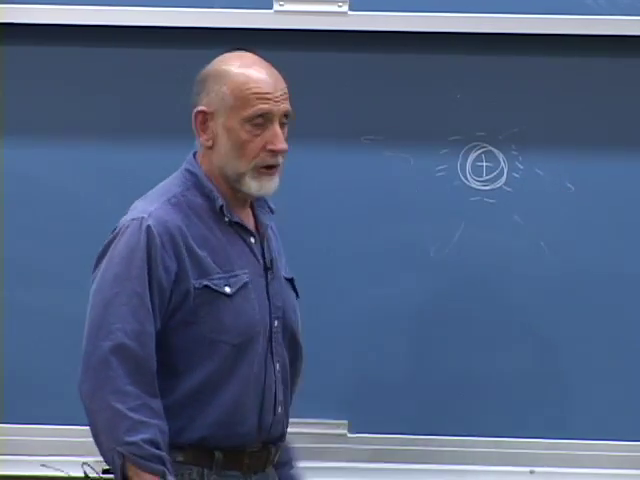
\includegraphics[width=0.82\textwidth]{lecture_10_figure_07.png}
\caption{導体の議論において、反対に帯電した遮蔽雲に囲まれた源電荷。}
\lectureframe{00:50:24}
\label{fig:l10-conductor-screening}
\end{figure}

\begin{classroomqa}
\audiencequestion{この再配置が遮蔽によって意味されるものか？\lecturetimestamp{00:51:25}}
\lecturerresponse{はい。雲より大きな距離では、挿入された電荷は遮蔽される。別の探針を雲の内側に持ち込むと、遮蔽の一部はもはや源と探針の間に位置できなくなる。すると、その下にある電荷はより強く現れる。}
\end{classroomqa}

雲は、可動電荷の力学と密度によって定まる特徴的なスケールをもつ。そのスケールより小さい\(r\)の間隔では、探針は雲を貫通する。したがって、
\begin{equation}
  F(r)\equiv\frac{e^2(r)}{4\pi r^2}.
  \label{eq:l10-running-charge-definition}
\end{equation}
を通じて走る電荷\(e(r)\)を定義してよい。理想化された導体では、\(e(r)\)は非常に長い距離でゼロに近づき、非常に短い距離で微視的な値に近づく。

\subsection{誘電体：部分的な遮蔽}

絶縁体では、電子は試料を横切る自由をもたず、原子に束縛されている。粗いが有用な模型は、各電子雲がそのイオンにばねで結びつけられていると描く。外部場がなければ、正と負の平均電荷中心は一致する。印加された場はそれらをわずかにずらし、双極子を誘起する。

負の源の周りでは、近くの電子雲は遠ざかるようにずれ、その正イオンをわずかに近くに残す。正の源の周りでは、それらは反対の向きにずれる。束縛電荷は源を完全に中和するほど遠くまで流れることができないので、長距離の場は消えるのではなく、誘電率によって減少する：
\begin{equation}
  V_{\mathrm{medium}}(r)
  =
  \frac{1}{\epsilon_r}
  \frac{e_1e_2}{4\pi\epsilon_0r}.
  \label{eq:l10-dielectric-coulomb}
\end{equation}
分極雲の内側の距離では、探針は再び裸の源をより多く見る。完全な遮蔽と部分的な遮蔽は、同じスケール依存の考えの二つの版である。

\section{分極可能な媒質としてのQED真空}

量子電磁力学の真空には物質的な原子はないが、荷電量子場がある。電子・陽電子のゆらぎは光子の伝播にループを寄与する。古いディラックの海の言葉では、電場は満たされた負エネルギー状態を歪める。現代の言葉では、真空分極が光子伝播関数を着飾る。媒質の描像は、仮想対が分極すると述べる。その正と負の成分は反対方向にずれる。

正の源は負の分極電荷の小さな過剰に囲まれ、負の源は正の分極電荷に囲まれる。したがって、遠くで測定される電荷は、未分解の源に結びつけるであろうパラメータより小さい。通常の物質と異なり、真空は連続的な運動量にわたるゆらぎを含む。低エネルギーの対はより長い距離の構造に対応し、高エネルギーの対はより短い距離を探る。過程が単純に止まる最終的な雲の半径は存在しない。

二つの電子をより近づけると、最も大きな分極雲が最初にそれらの間に収まらなくなる。それらを近づけると、次々により小さな雲が剥がれていく。有効な電気結合は、逆距離とともに対数的に、あるいは同等にエネルギーとともに増大する：
\begin{equation}
  \alpha(Q)
  \simeq
  \frac{\alpha(\mu)}
  {1-\dfrac{2\alpha(\mu)}{3\pi}
  \ln\!\left(\dfrac{Q}{\mu}\right)}
  \label{eq:l10-qed-running}
\end{equation}
その閾値より十分上の一つの荷電ディラックフェルミオンについて、主要次数で。追加の荷電種は、それらの閾値を越えると係数を変える。

\begin{figure}[htbp]
\centering
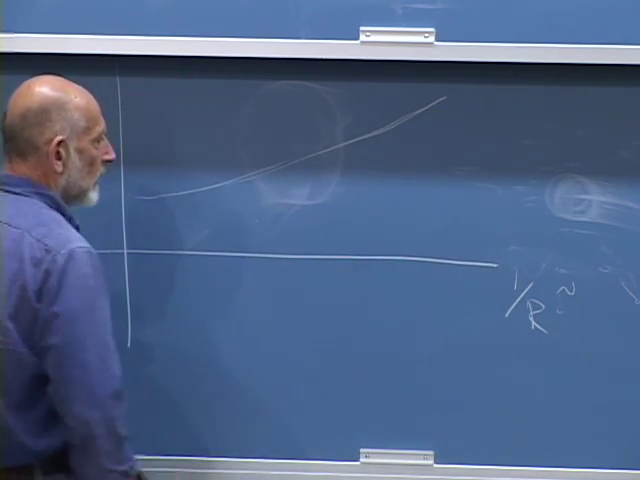
\includegraphics[width=0.82\textwidth]{lecture_10_figure_08.png}
\caption{QEDの有効電荷は、水平スケール\(1/R\)、したがって探るエネルギーが増大するにつれて、ゆっくりと増大する。}
\lectureframe{01:02:13}
\label{fig:l10-qed-running-board}
\end{figure}

電子散乱がその操作的版を与える。より高い衝突エネルギーはより短いド・ブロイ波長とより小さい最近接距離を意味する。したがって振幅は、その運動量移行に適した結合定数を用いなければならず、すべてのスケールに対して一つの固定した数を用いるのではない。

\begin{classroomqa}
\audiencequestion{ランニングが初めて測定可能になるのはどの距離においてか。\lecturetimestamp{01:03:54}}
\lecturerresponse{電子の真空偏極は電子のコンプトンスケール付近、\(\lambda_C=\hbar/(m_ec)\)、すなわち換算波長でおよそ\(4\times10^{-11}\,\mathrm{cm}\)で重要になる。この効果は小さく対数的であるため、精度が必要である。より重い荷電粒子はそれぞれ自身の閾値においてランニングに加わる。}
\end{classroomqa}

\begin{classroomqa}
\audiencequestion{最小距離について語ることは、そこで何が起こるかをすでに知っていると仮定しているのか。\lecturetimestamp{01:04:49}}
\lecturerresponse{いいえ。我々は、その粒子内容と相互作用が有効である限りにおいてのみ理論を外挿する。新しい物理はランニングを変えうる。実験は、QEDが任意に短い距離まで完全な記述であり続けることを我々に告げてはいない。}
\end{classroomqa}

\begin{classroomqa}
\audiencequestion{グルーオンについては、スケール依存性は逆か。なぜか。\lecturetimestamp{01:05:03}}
\lecturerresponse{はい。クォークループは荷電物質に類似した仕方で色荷を遮蔽するが、グルーオン自身が色を担い、非線形に相互作用する。それらの寄与は逆の符号をもち、観測されたクォークのフレーバー数に対して支配的である。その結果は反遮蔽と漸近的自由である。}
\end{classroomqa}

\begin{classroomqa}
\audiencequestion{それが無限に小さい距離を必要とするならば、裸の電荷をどのようにして決定できるのか。\lecturetimestamp{01:05:28}}
\lecturerresponse{一意な、正則化に依存しない裸の電荷を直接測定することはない。選ばれた短距離カットオフまたは繰り込みスケールにおいてパラメータを定義し、測定された低エネルギー量が固定されたままになるようにそれを調整する。スケール依存の繰り込み結合定数が有用な物理的対象である。}
\end{classroomqa}

\begin{classroomqa}
\audiencequestion{QEDの電荷は無限エネルギーの極限で有限の値に近づくのか。\lecturetimestamp{01:05:39}}
\lecturerresponse{それ自体で外挿された摂動的QEDにおいてはそうではない。その正のベータ関数は結合定数を対数的に増大し続けさせ、形式的には途方もなく高いスケールにおけるランダウ極に導く。その形式的な極を物理的であると扱うよりずっと前に、この記述は電弱理論に埋め込まれ、最終的にはさらなる物理によって変更されると期待される。}
\end{classroomqa}

\subsection{繰り込みが変えるものと保つもの}

カットオフ長\(a\)を選び、対応する入力を\(e(a)\)と呼び、固定された長距離の観測量を計算する。異なるカットオフ\(a'\)も、同じ観測量が再現されるように入力を\(e(a')\)に変えるならば、同様に受け入れられる：
\begin{equation}
  \frac{d}{d\ln\mu}\,\mathcal O_{\mathrm{physical}}=0,
  \qquad
  \mu\frac{de}{d\mu}=\beta(e).
  \label{eq:l10-rg-invariance}
\end{equation}
その補償的な流れが繰り込み群である。

\begin{classroomqa}
\audiencequestion{裸という語は特にプランク長を指さなければならないのか。\lecturetimestamp{01:06:20}}
\lecturerresponse{いいえ。任意に選ばれたカットオフで記述を打ち切り、そこのパラメータを裸と呼んでよい。そのパラメータを適切に変えながらカットオフを変えることは、アクセス可能な物理を変えないままにする。プランク長は、通常の量子場の理論が置き換えられなければならないもっともらしい場所であり、繰り込みに要求される規約ではない。}
\end{classroomqa}

\begin{classroomqa}
\audiencequestion{この手続きは、ズームインして記述を減衰させることの問題なのか。\lecturetimestamp{01:07:15}}
\lecturerresponse{概念的にはズームインすることである。我々は、固定された実験的にアクセス可能な波長における予測が同じままであるために、より細かい記述のパラメータがどのように変わる必要があるかを問う。}
\end{classroomqa}

\begin{classroomqa}
\audiencequestion{同じランニング現象は重力でも起こるのか。\lecturetimestamp{01:08:14}}
\lecturerresponse{重力にもスケール依存性はあるが、単純に同じ誘電的遮蔽の機構ではない。本講義にとっては次元解析で十分である：局在化はエネルギーを高め、エネルギーは重力を及ぼし、その結果生じる無次元の重力強度はエネルギーとともに急速に増大する。}
\end{classroomqa}

\section{QCD：反遮蔽、フラックス管、漸近的自由}

ハドロン的距離では、クロモ電場の力線は電磁的なクーロン場のように球対称に広がらない。グルーオンの自己相互作用がそれらをクォークと反クォークの間の狭い管に絞り込む。管が単位長さあたりほぼ一定のエネルギー\(\sigma\)をもつならば、
\begin{equation}
  V_{q\bar q}(r)
  \simeq
  -\frac{C_F\alpha_s(r)}{r}
  +\sigma r .
  \label{eq:l10-cornell-potential}
\end{equation}
大きな\(r\)では、線形項が支配的である。対を引き伸ばすことは、タフィーのひもを引っ張るように、管をより多く生成し、エネルギーはゼロに近づくのではなく増大する。これがこの話の閉じ込めの側面である。

\begin{figure}[htbp]
\centering
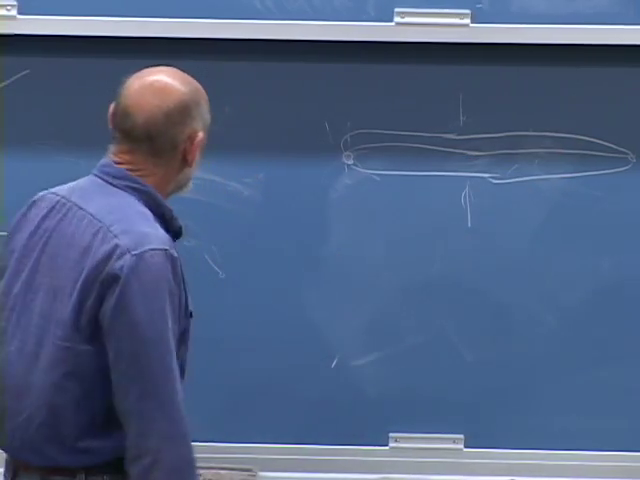
\includegraphics[width=0.84\textwidth]{lecture_10_figure_09.png}
\caption{クロモ電場の力線は、自由に広がるクーロン場としてではなく、離れた色源を結ぶ管として描かれる。}
\lectureframe{01:09:56}
\label{fig:l10-qcd-flux-tube-board}
\end{figure}

管の半径より短い距離では、ポテンシャルは近似的にクーロン形に戻るが、その結合はエネルギーとともに減少する。1ループでは、
\begin{equation}
  \alpha_s(Q)
  =
  \frac{4\pi}
  {\left(11-\frac23n_f\right)
  \ln(Q^2/\Lambda_{\mathrm{QCD}}^2)} .
  \label{eq:l10-asymptotic-freedom}
\end{equation}
\(n_f<17\) に対して係数は正であり、\(Q\to\infty\) のとき \(\alpha_s(Q)\to0\) となる。QCDは非常に短い距離では弱く、長い距離では強い。これは、講義で述べた逆の振る舞いの、走る結合定数による正確な表現である。

\begin{classroomqa}
\audiencequestion{QED曲線とQCD曲線の間で、弱い結合はどうなるのか。\lecturetimestamp{01:11:53}}
\lecturerresponse{その走りは中間的であり、どの電弱因子を追うかによって異なる。電弱スケールより上では、適切な量は \(U(1)_Y\) 結合と \(SU(2)_L\) 結合である。一方は上昇し、他方はゆっくり下降する。下降する強い結合と合わせると、それらの外挿値は高エネルギーで驚くほど近づく。}
\end{classroomqa}

\section{統一へ向かって走る}

弱いスケール付近で3つのゲージ結合を測定し、提案された理論の粒子内容でそれらを発展させる。すべてのベータ関数は対数的であるため、エネルギーの巨大な変化は結合の適度な変化しか生まない。標準模型の軌跡は互いに近づくが、正確には一致しない。最小超対称標準模型の低エネルギー粒子内容では、1ループの軌跡は
\begin{equation}
  M_{\mathrm{GUT}}\sim10^{16}\,\mathrm{GeV}.
  \label{eq:l10-gut-scale}
\end{equation}
付近ではるかに近くで一致する。

このプロットは証拠であり、証明ではない。未発見粒子からの閾値、高次ループ補正、統一理論の詳細が曲線をずらす。2010年の講義は、超対称スペクトルにおけるおよそパーセントレベルの収束を強調している。それは弱いスケールの超対称性を特に魅力的にしたからである。コライダーエネルギーで超対称パートナーが存在しないことは、今やそのスペクトルの最も単純な版が当初期待されたようには実現していないことを意味する。精密統一は依然として模型に依存する。

\begin{figure}[htbp]
\centering
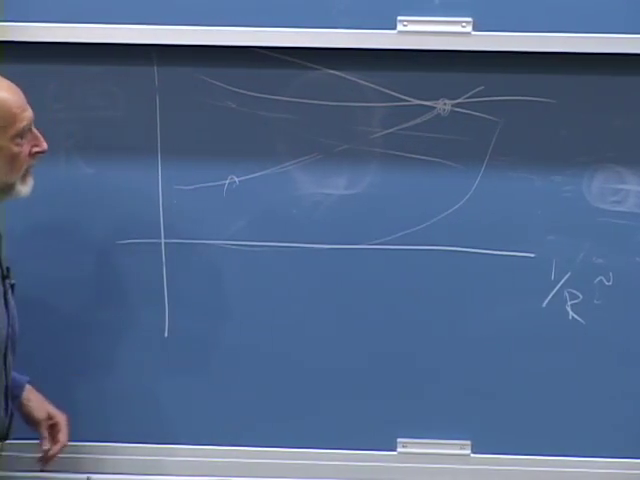
\includegraphics[width=0.84\textwidth]{lecture_10_figure_10.png}
\caption{黒板の定性的な結合プロット：強い曲線は下降し、電弱曲線はゆっくりとそれに向かって発展し、重力は遠紫外付近で急激に上昇する。}
\lectureframe{01:16:29}
\label{fig:l10-unification-board}
\end{figure}

なぜ出会いの点の近傍を基本的とみなすのか。そこでは入力が最も単純になりうるからである。3つの無関係な低エネルギー結合は、単一のゲージ群に対応する1つの高エネルギー結合の、異なるドレスされた子孫でありうる。これが、先の \(SU(5)\) の問いの背後にある数値的な手がかりである。

重力は同じ対数スケッチ上で、はるかに速く上昇する曲線として現れる。それはGUTスケールで正確にゲージ曲線と交差するわけではないが、数十年分のエネルギー範囲内で1の桁になる。対数軸上では、その近さは示唆的である。\(10^{16}\)、\(10^{17}\)、\(10^{18}\)、そして \(10^{19}\,\mathrm{GeV}\) は、いずれかが電弱スケールに近いよりもはるかに互いに近い。

\section{なぜ重力は短距離で強くなるのか}

\subsection{静止質量だけでなくエネルギーが重力を生む}

ゆっくり動く2つの質量の間のニュートンの力は
\begin{equation}
  F_G=\frac{Gm_1m_2}{r^2}.
  \label{eq:l10-newton-force}
\end{equation}
相対論的な次元評価では、各静止質量を対応するエネルギーを \(c^2\) で割ったものに置き換える：
\begin{equation}
  F_G(r)\sim\frac{GE_1E_2}{c^4r^2}.
  \label{eq:l10-relativistic-gravity-force}
\end{equation}
これは一般相対論の代わりではない。応力、運動量の流れ、圧力もまた重力の源となる。これは当面の問いに対する正しいスケーリング評価である。

各粒子を大きさ \(r\) の領域に局在化させる。不確定性原理は
\begin{equation}
  p\sim\frac{\hbar}{r}.
  \label{eq:l10-localization-momentum}
\end{equation}
を要求する。十分に小さい \(r\) では、運動量は超相対論的であるので、
\begin{equation}
  E\simeq pc\sim\frac{\hbar c}{r}.
  \label{eq:l10-localization-energy}
\end{equation}
そのような2つのエネルギーを
\eqref{eq:l10-relativistic-gravity-force}
に代入すると
\begin{equation}
  F_G(r)
  \sim
  \frac{G\hbar^2}{c^2r^4}.
  \label{eq:l10-short-distance-gravity-force}
\end{equation}
が得られる。対応するポテンシャルエネルギーのスケールは
\begin{equation}
  U_G(r)\sim-\frac{G\hbar^2}{c^2r^3}.
  \label{eq:l10-short-distance-gravity-potential}
\end{equation}
である。これがライブ計算中に訂正された区別である。ポテンシャルは \(1/r^3\) でスケールし、力は \(1/r^4\) でスケールする。

\begin{classroomqa}
\audiencequestion{超相対論的粒子に対して、エネルギーは
\(p^2/(2m)\)
か。\lecturetimestamp{01:22:18}}
\lecturerresponse{いいえ。それは非相対論的な式である。
\(E^2=p^2c^2+m^2c^4\)
から、極限 \(pc\gg mc^2\) は
\(E\simeq pc\)
を与える。\(p\sim\hbar/r\) と組み合わせると、局在化エネルギーは
\(\hbar c/r\)
である。}
\end{classroomqa}

\begin{figure}[htbp]
\centering
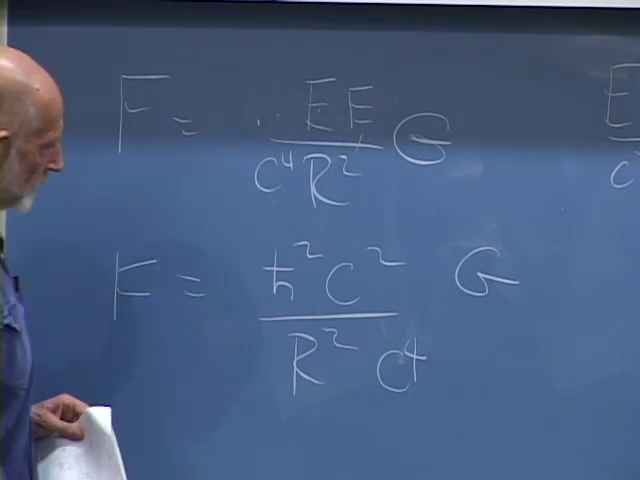
\includegraphics[width=0.84\textwidth]{lecture_10_figure_11.png}
\caption{黒板では、\(c\) と \(r\) の冪を確認しながら、相対論的エネルギーをニュートンの法則に代入している。}
\lectureframe{01:23:29}
\label{fig:l10-gravity-derivation-board}
\end{figure}

\begin{classroomqa}
\audiencequestion{\(c\) の因子は相殺されたのか、そして主張された
\(1/r^3\)
の法則は力の法則だったのか。\lecturetimestamp{01:23:38}}
\lecturerresponse{黒板の計算はリアルタイムで訂正される。2つの有効質量は \(E_1E_2/c^4\) に寄与する。
\(E_i\sim\hbar c/r\)
とすると、分母には \(c\) の2つの冪が残る。結果として得られる力は \(G\hbar^2/(c^2r^4)\) である。\(1/r^3\) の式はポテンシャルエネルギーに属する。}
\end{classroomqa}

\begin{classroomqa}
\audiencequestion{ここで議論している重力は引力である、
正しいか。\lecturetimestamp{01:24:42}}
\lecturerresponse{はい。上の式は大きさを表している。ニュートン重力ポテンシャルは正のエネルギーに対して負符号をもつので、この見積もりでは力は引力である。}
\end{classroomqa}

\begin{classroomqa}
\audiencequestion{局在化がエネルギーを高めるために重力が相対的に強くなり、一方で電荷自体は同じ運動学的因子を得ない、ということでよいか。\lecturetimestamp{01:25:02}}
\lecturerresponse{そのとおり。エネルギーが重力電荷である。量子状態を圧縮すると運動量とエネルギーが高まり、したがって重力の源となるものも高まる。電荷は無次元であり、はるかに遅い対数くりこみを別にすれば、その直接の\(1/r\)因子を獲得しない。}
\end{classroomqa}

\subsection{プランク交差}

自然単位で1程度の電荷の間にはたらく電磁気力の大きさは
\begin{equation}
  F_{\mathrm{EM}}(r)
  \sim
  \alpha\,\frac{\hbar c}{r^2}.
  \label{eq:l10-em-force-alpha}
\end{equation}
である。これを\eqref{eq:l10-short-distance-gravity-force}と等置すると
\begin{equation}
  r^2\sim\frac{G\hbar}{\alpha c^3}.
  \label{eq:l10-gravity-em-crossing}
\end{equation}
が得られる。講義では、基本的な重力の長さを明らかにするために、無次元のゲージ因子を1程度に設定する：
\begin{equation}
  \boxed{\ell_P=\sqrt{\frac{\hbar G}{c^3}}}
  \simeq1.616\times10^{-35}\,\mathrm{m}.
  \label{eq:l10-planck-length}
\end{equation}
実際の\(\alpha\)を保つと、電磁気力との等置は1程度の対数スケール因子\(r\sim\ell_P/\sqrt\alpha\)だけずれる。基本的な主張は自然単位でより簡潔である：
\begin{equation}
\begin{aligned}
  \alpha_G(E)
  &\equiv\frac{GE^2}{\hbar c^5}
  =\left(\frac{E}{E_P}\right)^2,
  \\
  E_P
  &=\sqrt{\frac{\hbar c^5}{G}}
  \simeq1.22\times10^{19}\,\mathrm{GeV}.
\end{aligned}
  \label{eq:l10-gravitational-coupling}
\end{equation}
重力は\(E\)が\(E_P\)に近づくと強くなる。

\begin{classroomqa}
\audiencequestion{比較で1に等しく設定されていたのは\(G\)か、それとも電気結合か。\lecturetimestamp{01:27:02}}
\lecturerresponse{電気結合は粗い見積もりのために1程度の数として扱われていた。ニュートンの定数は残らなければならない。それはプランクスケールを決める次元をもつ量である。}
\end{classroomqa}

\begin{classroomqa}
\audiencequestion{\(r\)、\(\hbar\)、\(c\)の中間の冪が次元的に整合していないように見える。修正された計算は何か。\lecturetimestamp{01:27:47}}
\lecturerresponse{最初からエネルギーを用いる。局在化により
\(E\sim\hbar c/r\)、したがって
\(U_G\sim GE^2/(c^4r)=G\hbar^2/(c^2r^3)\)が得られる。これを
\(U_{\mathrm{EM}}\sim\alpha\hbar c/r\)と比較する。
\(\alpha\)を1程度に設定すると
\(r^2=G\hbar/c^3\)が得られる。講義と板書は
\(r=\sqrt{G\hbar/c^3}\)、すなわちプランク長に到達する。}
\end{classroomqa}

\begin{figure}[htbp]
\centering
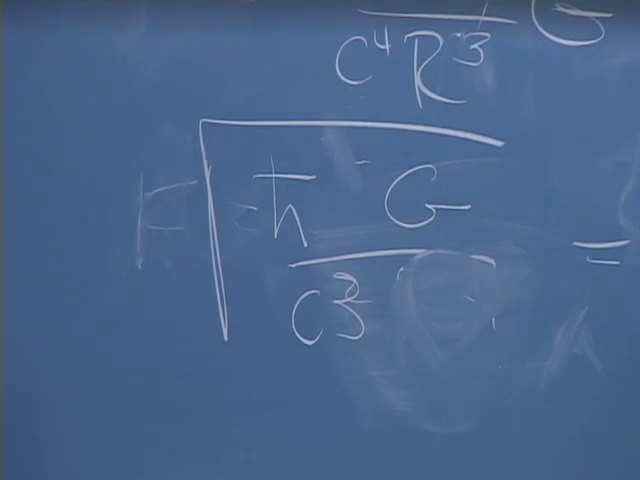
\includegraphics[width=0.84\textwidth]{lecture_10_figure_12.png}
\caption{実時間の次元検査の修正された終点：
\(r=\sqrt{\hbar G/c^3}\)。}
\lectureframe{01:32:16}
\label{fig:l10-planck-length-board}
\end{figure}

\section{階層性問題の再登場}

ゲージ結合は非常に高いスケール付近で同程度になり、重力はプランクスケール付近で強くなる。これらの巨大なスケールは今や、恣意的な大きな数というよりも、微視的記述が簡単になる場所のように見える。それらに対して、電弱真空期待値\(F\)は異常に小さい：
\begin{equation}
  \frac{v}{E_P}\sim2\times10^{-17}
  \label{eq:l10-electroweak-planck-ratio}
\end{equation}
ここで\(c=1\)の単位を用いる。プランクスケールの代わりに大統一スケールを用いると、正確な比は変わるが、謎は変わらない。

\(F\)が小さければ、\(W\)、\(Z\)、荷電レプトン、クォークの質量は、ゲージ対称性によってその質量がそれに比例するため、それに従う。その保護がない粒子は重いままでいられる。したがって、未解決の問いは、なぜすべての既知の質量が独立に微小なのかということではない。なぜヒッグスセクターがこのただ一つの微小な対称性の破れのスケールを与えるのかということである。

\begin{classroomqa}
\audiencequestion{もし\(F\)を計算できたなら、他のすべての質量も計算可能になるのか。\lecturetimestamp{01:34:39}}
\lecturerresponse{それは全体的な電弱スケールを決定し、ゲージ結合と湯川結合が与えられれば、対応する粒子質量を決定する。残る問題は、通常の紫外発散に敏感な計算が、対称性または力学的機構がそれを保護しない限り、ヒッグス質量パラメータを高い基礎スケールへと押しやる傾向があることである。}
\end{classroomqa}

微調整という言葉はその感受性を予期している。カットオフ記述では、スカラー質量パラメータはおおよそ次の形の補正を受ける
\begin{equation}
  \delta\mu^2
  \sim
  \frac{C}{16\pi^2}\Lambda^2,
  \label{eq:l10-higgs-quadratic-sensitivity}
\end{equation}
ここで\(C\)はゲージ結合、湯川結合、スカラー結合をまとめたものであり、\(\Lambda\)は有効理論が置き換えられるスケールを表す。もし\(\Lambda\)が大統一スケールまたはプランクスケール付近であれば、
\(\mu^2\sim v^2\)を得るには、入力と輻射補正の間に非常に精密な相殺が必要であるように見える。これがゲージ階層性問題の自然性の形である。これは講義が次の四半期に約束する計算の編集上の補完であり、特定の正則化依存の産物自体が観測可能であるという主張ではない。

\begin{classroomqa}
\audiencequestion{プランク長は最終的な遮蔽雲の半径として視覚化されるべきか。\lecturetimestamp{01:35:03}}
\lecturerresponse{いいえ。誘電体的描像はゲージ電荷のくりこみを説明するが、プランクの議論は局在化エネルギーと次元をもつ重力結合を用いた。この導出には文字通りの重力遮蔽雲は存在しない。}
\end{classroomqa}

\subsection{相互作用についての最後の問い}

最後の数分は、ヒッグスポテンシャルと、ラグランジアンがどのような項を含みうるかに戻る。

\begin{classroomqa}
\audiencequestion{ヒッグスポテンシャルは\(\phi^6\)を含んでもなお対称性を保てるだろうか。\lecturetimestamp{01:35:20}}
\lecturerresponse{はい。偶数乗はおもちゃの\(\phi\mapsto-\phi\)対称性を保つが、\(\phi^5\)はそれを破るであろう。4次元では\(\phi^6\)の係数は負の質量次元をもつので、その項は高いスケール、たとえば\(c_6\phi^6/\Lambda^2\)によって抑制される。これはパワーカウンティングで繰り込み可能ではないが、有効な相互作用としては妥当である。}
\end{classroomqa}

\begin{classroomqa}
\audiencequestion{ヒッグス場の冪は生成と消滅の過程を表すのか、したがって\(\phi^4\)はヒッグス-ヒッグス散乱を予言するのか。\lecturetimestamp{01:35:52}}
\lecturerresponse{はい。真空のまわりで展開した後、量子化された場の冪は頂点を生成する。四次の項には四本のヒッグス頂点が含まれ、シフトされたポテンシャルは三次の相互作用も生み出す。それらの係数を知ることで、通常のダイヤグラム計算に従い、\(hh\to hh\)のような過程を予言できる。}
\end{classroomqa}

\begin{classroomqa}
\audiencequestion{基礎的なラグランジアンは、その場について多項式であり、4乗より高い冪を含んではならないのだろうか。\lecturetimestamp{01:36:09}}
\lecturerresponse{摂動的に繰り込み可能な4次元スカラー理論では、次元が最大4までの演算子が伝統的な有限のリストをなす。現代の有効場の理論はそれほど制限的ではなく、より高次元の演算子が許され、短距離の物理を記述するが、その効果は高いスケールの冪によって抑制される。したがって、時折の例外は古い規則にとって本質的である。}
\end{classroomqa}

\begin{classroomqa}
\audiencequestion{自己相互作用の項は、結合定数の走りの議論から省略されていたのだろうか。\lecturetimestamp{01:36:44}}
\lecturerresponse{それらは概念的に含まれていた。グルーオンの自己相互作用こそが、QEDに対して符号を逆転させ、反遮蔽を生み出すものである。同様にヒッグスの自己相互作用は、スカラーおよび他の標準模型パラメータの走りに寄与する。}
\end{classroomqa}

\begin{classroomqa}
\audiencequestion{異なる相互作用が互いの走りに影響を与える交差項はあるのだろうか。\lecturetimestamp{01:37:23}}
\lecturerresponse{はい。より高次のループ次数では、ベータ関数はゲージ結合、湯川結合、スカラー結合の混合積を含む。それらの無次元結合が十分小さい間は摂動論は有用であり続ける。なぜなら、 successive なループ次数はそれに対応して抑制されるからである。}
\end{classroomqa}

\begin{classroomqa}
\audiencequestion{\(F\)が微調整されていると言うとき、正確には何が意味されていたのか。\lecturetimestamp{01:37:44}}
\lecturerresponse{完全な答えは講義では先延ばしにされる。問題は、軽いスカラースケールがはるかに大きな紫外寄与に対して不安定であることであり、それは\eqref{eq:l10-higgs-quadratic-sensitivity}によって要約される。超対称性は相殺を強制するために提案された一つの方法であったが、階層性問題自体は確認された解決策を選び出すものではない。}
\end{classroomqa}

\begin{classroomqa}
\audiencequestion{繰り込み群自体を今説明できるだろうか。\lecturetimestamp{01:37:56}}
\lecturerresponse{残りの数分ではできない。その作用的内容はすでに現れている。分解能を変え、結合定数を流し、固定された物理的予言を保つことである。完全な扱いはコースの次の段階に属する。}
\end{classroomqa}

そこが、この一連の流れが適切に我々を残す場所である。ヒッグス機構は標準模型を内部的に首尾一貫させた。それはカイラルゲージ対称性を保ち、弱ゲージボソンとフェルミオンに質量を与え、物理的なヒッグス相互作用を予言する。次に繰り込みは、それらの相互作用がスケールとともにどのように変化するかを教え、ゲージ力が統一された起源を共有するかもしれないことを示唆する。重力は独立した議論によって第二の高いスケールを供給する。これらの成功のいずれも、ヒッグス真空期待値がなぜ両方よりもはるかに低いのかを説明しない。したがって最終講義は主題を閉じるのではなく、次の主題が集中すべき小さな数を特定する。